\documentclass{article}
\usepackage[utf8]{inputenc}

\title{623 Project 3: Discontinuous Galerkin Finite Element Solver}
\author{Josh Anibal}
\date{April 5th 2019}

\usepackage{natbib}
\usepackage{graphicx}
\usepackage{pdflscape}
\usepackage{afterpage}
\usepackage{lscape}
\usepackage{amsmath, esint}
\usepackage{geometry}
\geometry{ margin=0.75in}
\usepackage[utf8]{inputenc}
\usepackage[english]{babel}

\usepackage{floatrow}

\usepackage[outdir=./]{epstopdf}
\usepackage[parfill]{parskip}
% \epstopdfsetup{outdir=./}
% Table float box with bottom caption, box width adjusted to content
\newfloatcommand{capbtabbox}{table}[][\FBwidth]
% \setlength\parindent{0pt}
\graphicspath{{../figures/}}

% \setlength{\parindent}{4em}
% \setlength{\parskip}{1em}
% \renewcommand{\baselinestretch}{2.0}
\usepackage{float}

\usepackage{booktabs}

\begin{document}
\label{Eqn:DE}
\maketitle

\section*{Introduction}
In this assignment we were tasked with using a discontinuous Galerkin (DG) finite element method (FEM) to solve the Euler equations for the flow field over a bump in a chanel.
In this report we will study the effect of the solution basis function order ($p$) on the convergence properties of key outputs and flow field.



\section{Methodology}

\subsection{Governing Equations}
	The Euler equations describe the conservation of mass, energy, and momentum for a compressible, inviscid fluid.
	% These equations are shown in a  compact form in Eqn \ref{eqn:Euler}



	\begin{equation}
		\frac{\partial \mathcal{\mathbf{u} }}   {\partial t}
		+ \nabla   \cdot \vec{\mathbf{F}}(\mathbf{u})  = \mathbf{0}
		\label{eqn:Euler}
	\end{equation}
	\begin{equation*}
		\mathbf{u} =
		\begin{bmatrix}
			\rho \\ \rho u \\ \rho v \\ \rho E
		\end{bmatrix}
		,
		\mathbf{\vec{F}} =
		\begin{bmatrix}
			\rho u \\ \rho u^2 + p \\ \rho uv \\ \rho u H
		\end{bmatrix}
	\end{equation*}

	By solving these equations numerically we can determine an approximate solution for the state of the fluid within the domain.


\subsection{Discretization}
	\subsubsection{Spatial}
	These equations were discretized spatially using the discontinuous Galerkin finite element method.
	With this method, the domain is discretized into elements, each of with set of basis functions.
	By selecting the coefficients on these basis functions, the solution can be represented continuously within each element.
	In this particular case a set of full-order Lagrange basis functions were used for the basis functions within each cell.
	One advantage of DG FEM is that  it can be used to theoretically achieve an arbitrary order of accuracy by selecting basis function of the corresponding order.

	The underlying equation solved by the finite element discretization can be determined by solving for the weak form of the governing PDE (the Euler Equations).
	Applying this process yields Equation \ref{eqn:weak}.
	\begin{equation}
		M_k\frac{d\mathbf{u}_k}{dt} + \mathbf{R}_k =  0
		\label{eqn:weak}
	\end{equation}


	$\mathbf{M}_{k}$ represents the mass matrix and is given by Equation \ref{eqn:mass}.


	\begin{equation}
		\left[\mathbf{M}_{k}\right]_{i, j}=\int_{\Omega_{k}} \phi_{k, i} \phi_{k, j} d \Omega
		\mathbf{R}_i = \oint\limits_{\partial{A}} \mathbf{\hat{F}} \cdot \vec{n} dl
		\label{eqn:mass}
	\end{equation}

	$\mathbf{R}_k$ represents the weighted residuals in each element and has a component related to the solution representation in the interior and at element edges as shown in Equation \ref{eqn:res}.
	\begin{equation}
		R_{k, i}=\underbrace{-\int_{\Omega_{k}} \nabla \phi_{k, i} \cdot \vec{F} d \Omega}_{\text interior}+ \underbrace{\int_{\partial \Omega_{k}} \phi_{k, i}^{+} \hat{F}\left(u^{+}, u^{-}, \vec{n}\right) dl}_{edge}
		\label{eqn:res}
	\end{equation}

	The component of the residual related to the edge contribution enforces coupling between the elements and adds convective stability.
	The calculation of this component requires a computational flux calculation; For this implementation of DG the Roe flux function was used.

	The Roe flux is given by Equation \ref{eqn:roe} and uses a Roe-averaged state ,$\mathbf{u}^{*}$, to upwind each wave.
	\begin{equation}
		\hat{\mathbf{F}}=\frac{1}{2}\left(\mathbf{F}_{L}+\mathbf{F}_{R}\right)-\frac{1}{2}\left|\frac{\partial \mathbf{F}}{\partial \mathbf{u}}\left(\mathbf{u}^{*}\right)\right|\left(\mathbf{u}_{R}-\mathbf{u}_{L}\right)
		\label{eqn:roe}
	\end{equation}

	\subsubsection{Time Integration}
	To solve for the steady state of the flow in the domain we will march the state of the system forward in time until the residuals fall to within some tolerance.

	To advance the solution in time we use the Jameson Runge Kutta method with 4 stages (JRK4) shown in Equation \ref{eqn:JRK} .
	This method is 4th order accuracy in time and helps maintain stability for the more accurate spacial descretizations.
	The advantage of the Jameson implementation of the Runge Kutta scheme is that it reduces the memory required by ensuring each stage only depends on the prior.
	Additional time integration schemes we tried, such as total variation diminishing Runge Kutta 2 and 3 , but JRK4 was found to preform the best for this specific problem.
	\begin{equation}
	\begin{aligned} u^{(1)} &=u_{n}+\frac{h}{4} L\left(u_{n}\right) \\ u^{(2)} &=u_{n}+\frac{h}{3} L\left(u^{(1)}\right) \\ u^{(3)} &=u_{n}+\frac{h}{2} L\left(u^{(2)}\right) \\ u_{n+1} &=u_{n}+h L\left(u^{(3)}\right) \end{aligned}
		\label{eqn:JRK}
	\end{equation}



	\subsubsection{Geometry}

	To get high-order accuracy in our solution, high-order geometry is required.
	More specifically to ensure the theoretical order of accuracy of the solution we need a geometry of one order higher than the solution.
	To represent a higher-order geometry we use a set of Lagrange basis functions to map points from reference space to global space for the elements along the wall.
	The coefficients of the basis functions are the nodes of the element with additional nodes added to match the exact geometry.
	The intermediate points (such as the quadrature points) are then determined by evaluating the sum of the Lagrange basis functions (Equation \ref{eqn:qbasis}).

	\begin{equation}
	\vec{x}=\sum_{i=1}^{3} \vec{x}_{i} \phi_{i}(\xi, \eta)
	\label{eqn:qbasis}
	\end{equation}

	A zoomed-in view of the geometry for the \texttt{bump0.gri} mesh is shown in Table \ref{tab:mesh} to highlight the differences caused by geometric order.
\begin{table}[H]
	\begin{center}
	\begin{tabular}{ c@{}c@{} }


		\hline
		\multicolumn{2}{@{}c@{}}{Linear ($q=1$)}\\


		\hline
		% \vspace{1mm}
		\vspace{0.1mm}\\
		\multicolumn{2}{@{}c@{}}{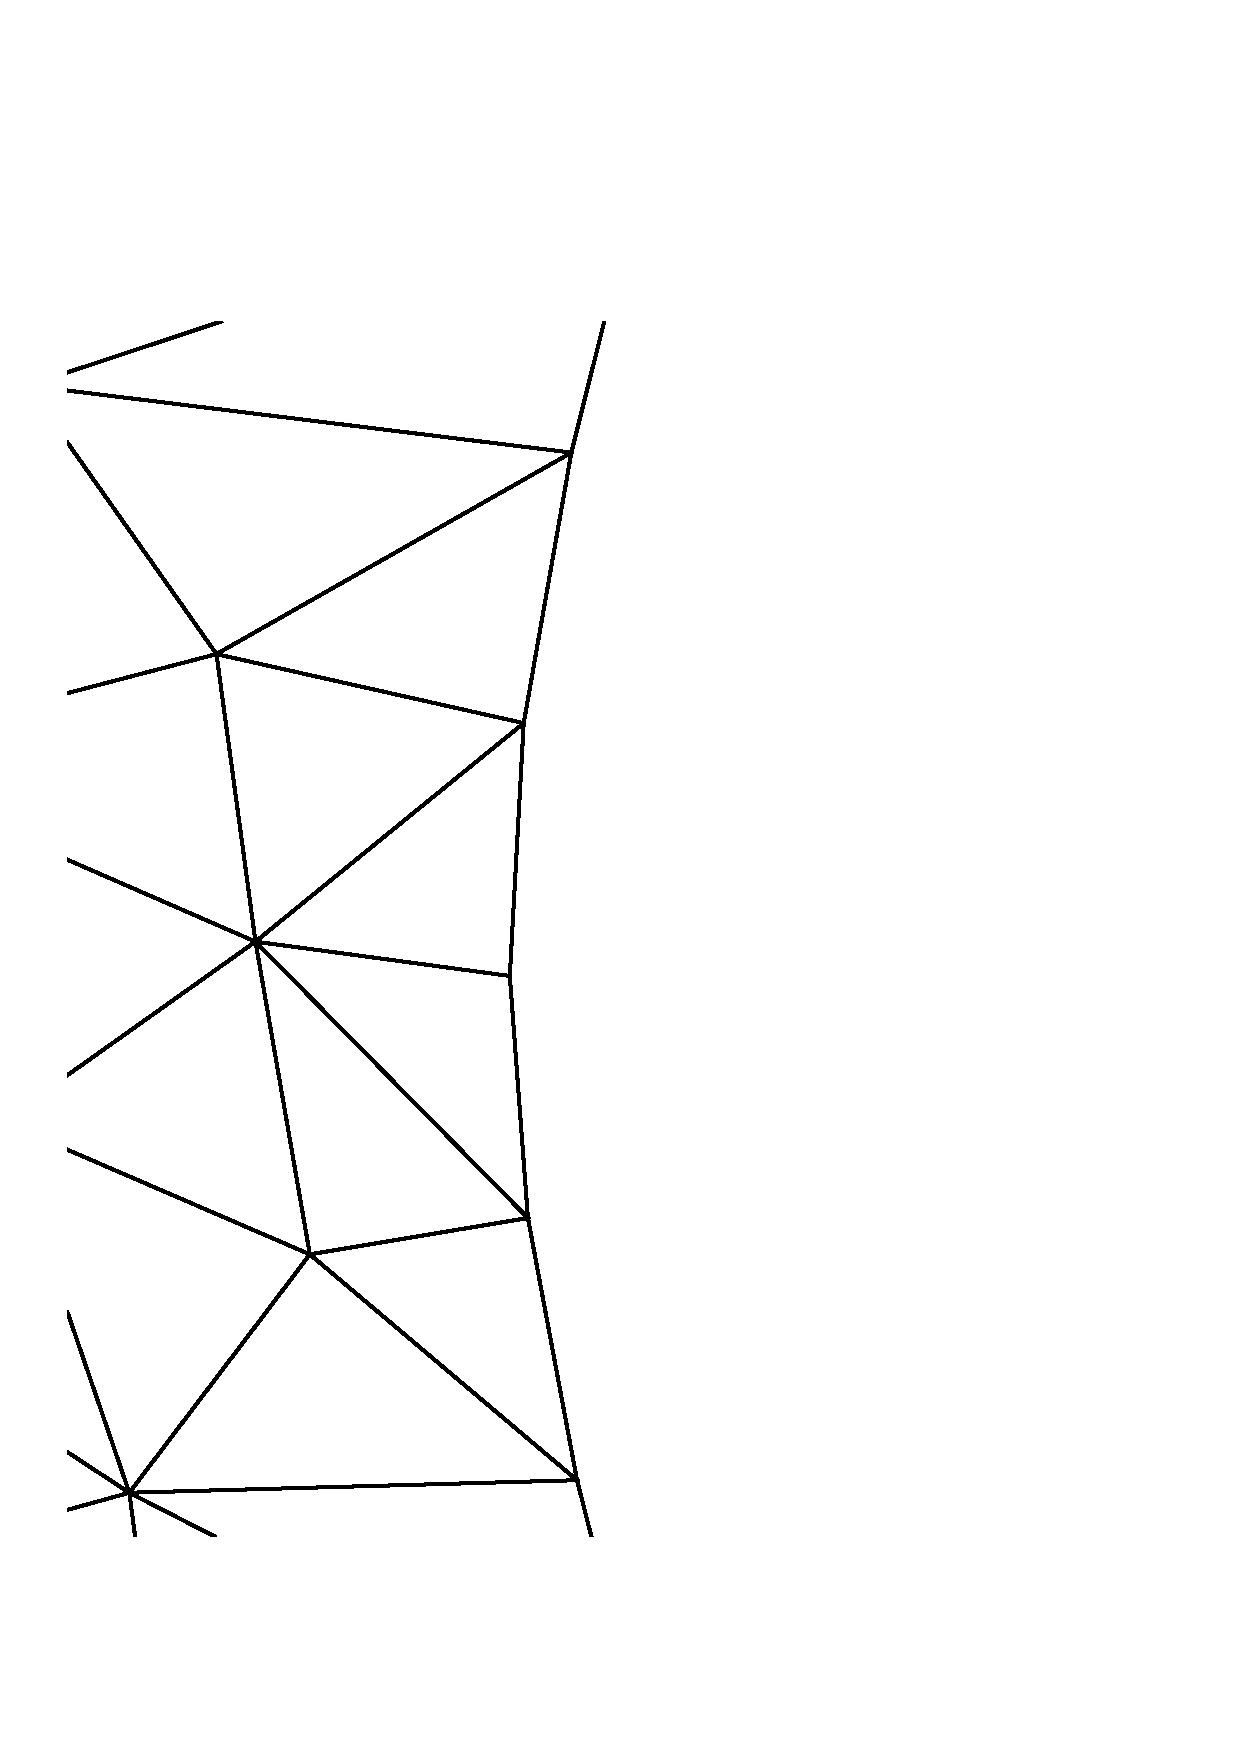
\includegraphics[width=0.75\textwidth,keepaspectratio]{bump0q1.pdf}}\\

		\hline
		\multicolumn{2}{@{}c@{}}{Quadratic ($q=2$)}\\

		\hline
		\vspace{0.1mm}\\

		\multicolumn{2}{@{}c@{}}{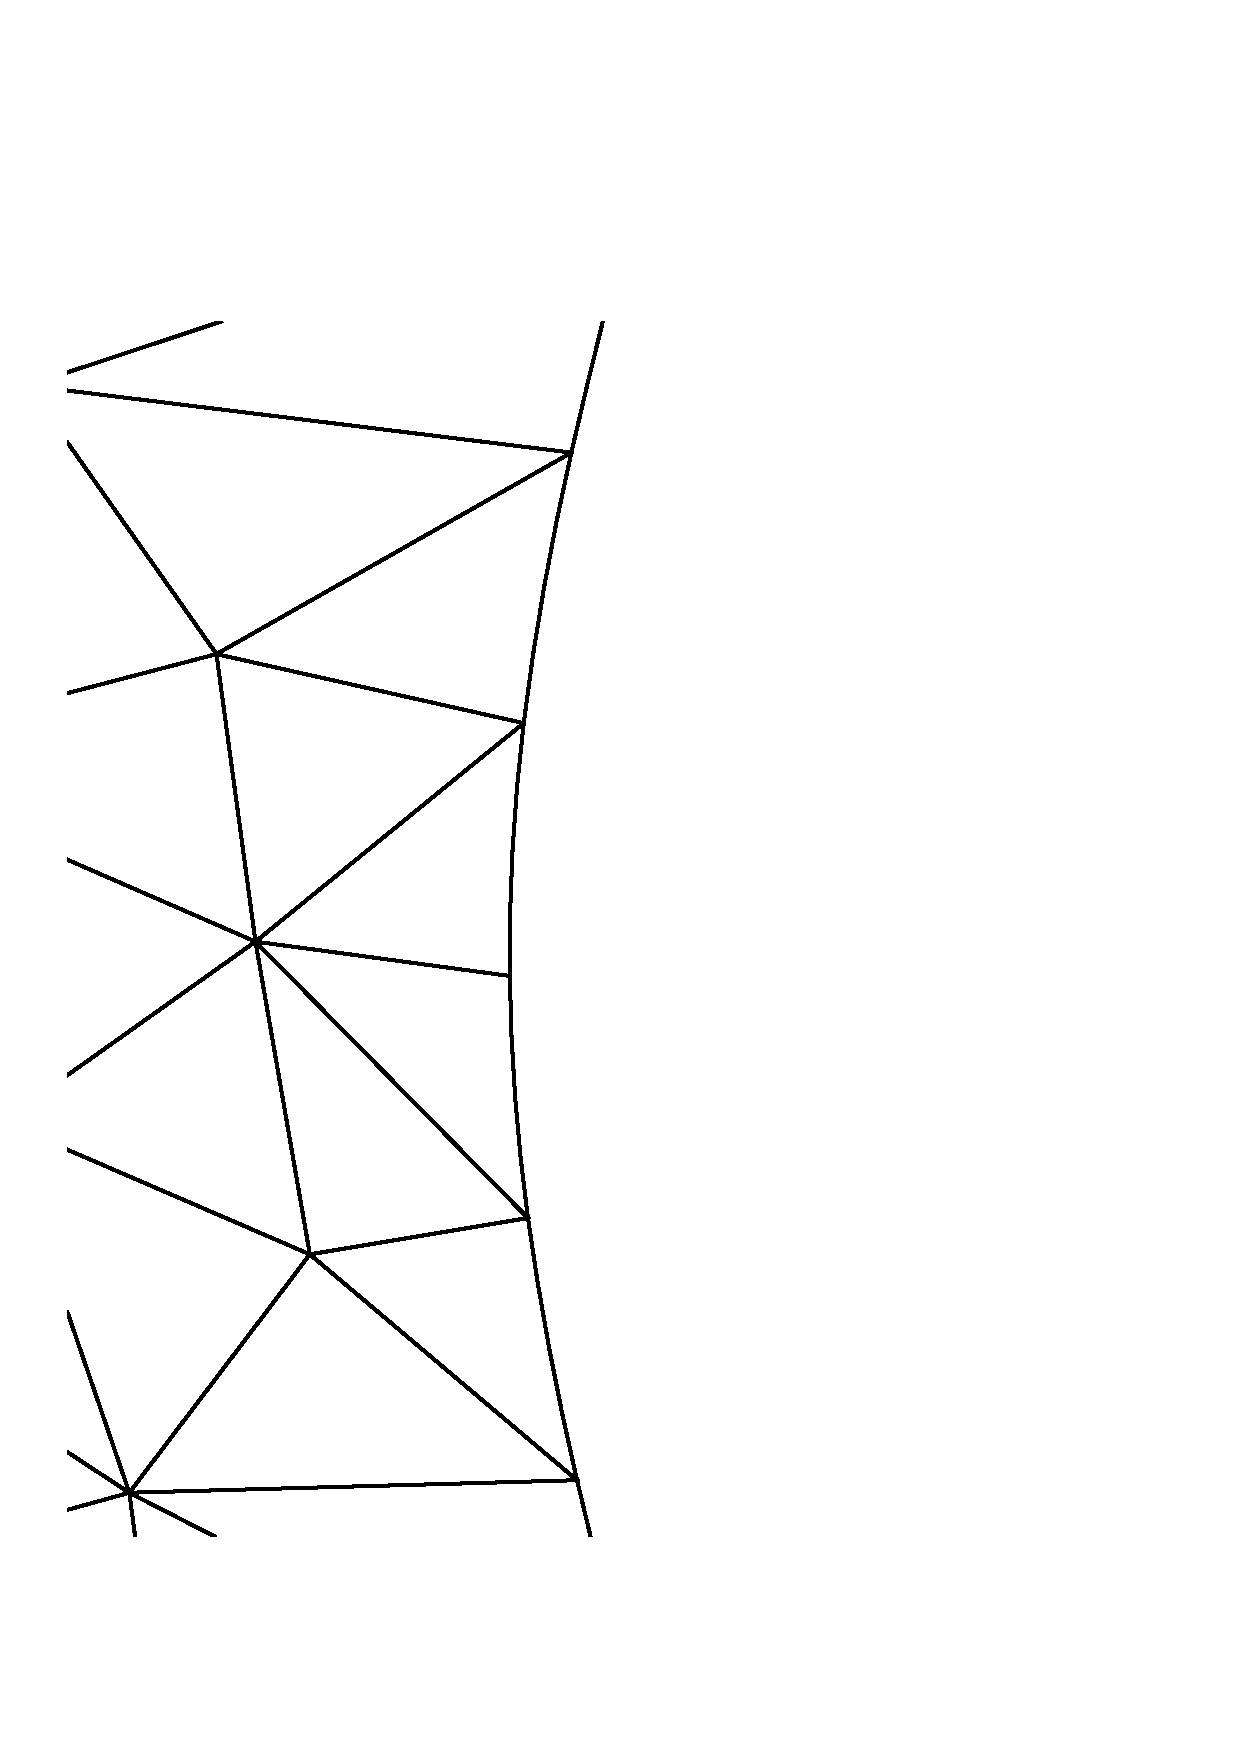
\includegraphics[width=0.75\textwidth,keepaspectratio]{bump0q2.pdf}}\\

		\hline
		\multicolumn{2}{@{}c@{}}{Cubic ($q=3$)}\\

		\hline
		\vspace{0.1mm}\\

		\multicolumn{2}{@{}c@{}}{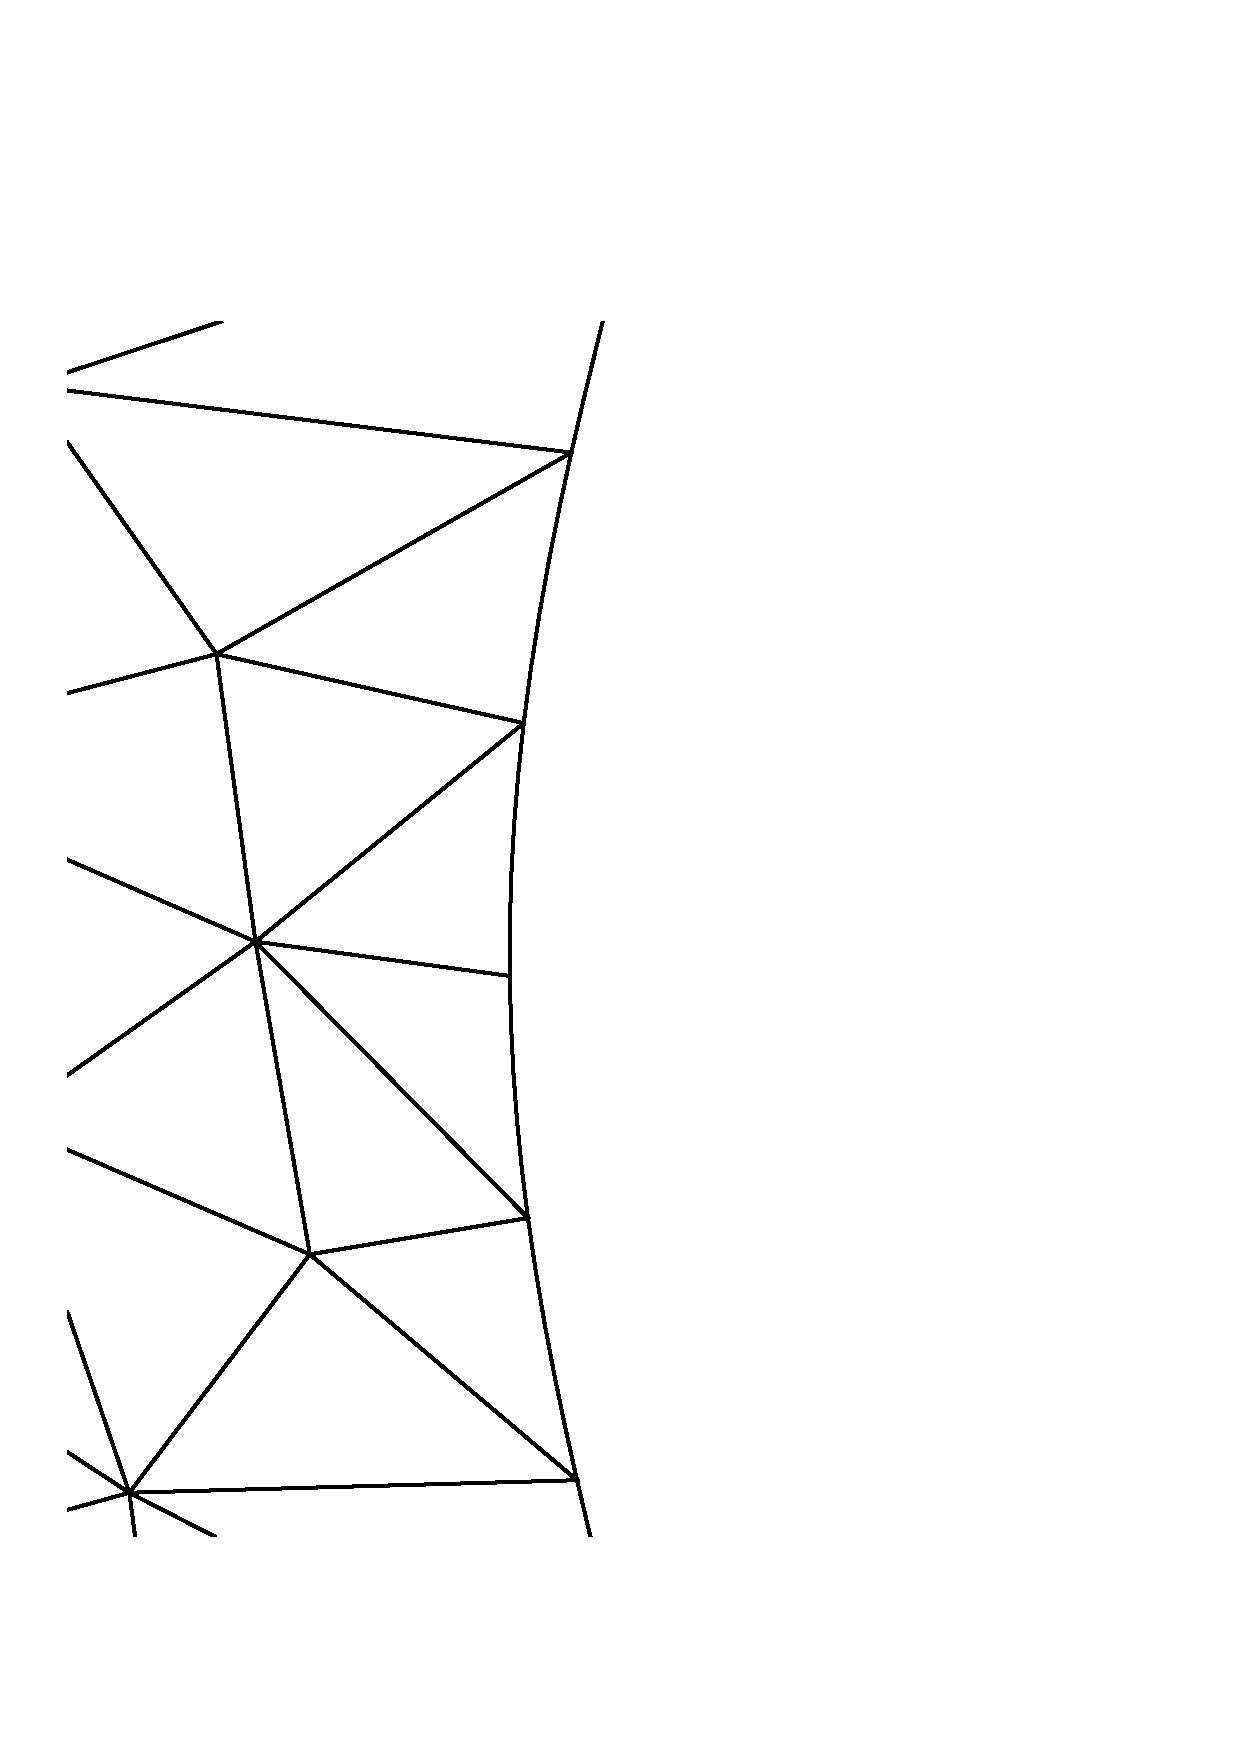
\includegraphics[width=0.75\textwidth,keepaspectratio]{bump0q3.pdf}}\\
		\vspace{0.25mm}\\
	\end{tabular}
	\caption{Geometric reparation of \texttt{bump0.gri} for the each geometric representation order}
	\label{tab:mesh}
	\vspace*{-3mm}
	\end{center}
\end{table}





\section{Accuracy Checks}
Before the code was used to solve for the actual flow field, a free stream residual and preservation test were preformed and an additional converge check.


\subsection{Residual Calculation}
To verify that the residuals were computed correctly all interior states were initialized to the free-stream state and the boundary condition fluxes were replaced using halo cells also set to the free-stream state.
The resulting residuals were on the order of machine precision, as expected, and are shown in Table \ref{tab:freestream}.


\begin{table}[H]
		\label{tab:freestream}
		\begin{tabular}{@{}llll@{}}
			\toprule
			& 0th Order& 1st Order & 2nd Order \\ \midrule
			$|R_{\infty}|$ & 2.2e-16  & 2.31e-15 & 4.247e-15  \\
			\bottomrule

		\caption{Residuals of the free-stream residual test}
		\end{tabular}
\end{table}

\subsection{Time Stepping}
A free-stream preservation test was performed to verify that the JRK4 methods was correctly updating the states.
The method was used to take 1,000 time steps and the starting and ending residual values are shown in Table 2.
Figure \ref{fig:free_stream} shows the residual at each iteration.
The residual for each methods hoovers around machine precision, with the exception of the 0th order method.
It is theorized that the residual of the 0th-order method stays constant because the initial residual was already at machine precision and then was multiplied by the inverse mass matrix and time step (both are less than 1 typically) before being used to calculate the next state causing under flow.

% The results of this test show that the residuals for both methods stay relatively constant over time as they should.
\begin{table}[H]
	\label{tab:fsp}
	\begin{tabular}{@{}llll@{}}
	\toprule
		& 0th Order& 1st Order & 2nd Order \\ \midrule
		Starting $|R_{\infty}|$ & 2.2e-16  & 2.31e-15 & 4.247e-15  \\
		Ending $|R_{\infty}|$ & 2.2e-16   & 4.72e-16 & 5.97e-16 \\
	\bottomrule
	\caption{Starting and ending residuals of the free-stream preservation test}

	\end{tabular}
\end{table}

\begin{figure}[H]
	\centering
	\includegraphics[width=0.60\textwidth,keepaspectratio]{freestream.png}
	\caption{Residual history for the free-stream preservation test}
	\label{fig:free_stream}
\end{figure}





\subsection{Convergence}

When we apply our methodology to the actual problem of the flow through a chanel with a bump, the residuals are indeed driven to zero.
Figure \ref{fig:res_history} shows the convergence history for each order on the \texttt{bump0.gri} mesh.
The 1st and 2nd order methods take approximately 4x and 18x the number of iterations to converge the solution to the same accuracy.
Additionally, the residuals for the 1st and 2nd order methods oscillate much more than that of the 0th order method.



\begin{figure}[H]
	\centering
	\includegraphics[width=0.60\textwidth,keepaspectratio]{converg.pdf}
	\caption{Residual history for \texttt{bump0.gri}}
	\label{fig:res_history}
\end{figure}

\subsection{Rates of Convergence}

The coefficient of lift ($C_l$), coefficient of drag $(C_d$), and integrated entropy error of the domain (Es) where calculated for each each solution order and the convergence of these values can be seen in Figures \ref{fig:conv_cl}, \ref{fig:conv_cd}, and \ref{fig:conv_Es} respectively.
The value of each quantity is plotted against the number of degrees of freedom (dof), which is total number of unknowns solved in the problem.
For the DG FEM the total number of degrees of freedom is simply the number of elements multiplied by the number of solution basis functions in each element.


The rate of convergence is included in each figure for convenience.
In general, the higher the solution order the faster the method converged toward the exactly value.
However this was not always the case, for example the 1st order method converged at a greater rate than the 2nd order method for both $C_l$ and $C_d$.
This is believed to have happened because of a possible inaccuracy in the "true" values for $C_l$ and $C_d$ as stated by Professor Fidkowski on Piazza.

\begin{figure}[H]
		\centering
		\includegraphics[width=0.60\textwidth,keepaspectratio]{conv_cd.png}
		\caption{Increasing the number of dof results in a more accurate $C_l$ estimation}
	\label{fig:conv_cl}
\end{figure}
\begin{figure}[H]
	\centering
	\includegraphics[width=0.60\textwidth,keepaspectratio]{conv_cl.png}
	\caption{Increasing the number of dof results in a more accurate $C_d$ estimation}
	\label{fig:conv_cd}
\end{figure}
\begin{figure}[H]
	\centering
	\includegraphics[width=0.60\textwidth,keepaspectratio]{conv_Es.png}
	\caption{The total entropy goes to zero with an increasing dof}
	\label{fig:conv_Es}
\end{figure}



\subsection{Run time}
For each combination of mesh refinement and solution order, the wall time was also measured and is shown in Figure \ref{fig:walltime}.
% For each accuracy level higher order methods
This comparison really highlights the advantage of the high-order DG methods.
For a given accuracy level the highest-order method is the quickest, and for a set time limit the highest-order method was the most accurate!

\begin{figure}[H]
	\centering
	\includegraphics[width=0.60\textwidth,keepaspectratio]{walltime.png}
	\caption{The highest-order methods is the quickest for a given level of accuracy}
	\label{fig:walltime}
\end{figure}





\subsection{Pressure Coefficient}
Figure \ref{fig:cp} shows the coefficient of pressure ($C_p$) along the lower wall for the \texttt{bump2.gri} mesh.
The 1st and 2nd-order methods produce a similar distribution that is more continuous and symmetric than the 0th order solution.

\begin{figure}[H]
	\centering
	\includegraphics[width=0.60\textwidth,keepaspectratio]{cp.png}
	\caption{The coefficient of pressure along the bump for each solution order}
	\label{fig:cp}
\end{figure}

Although the 1st and 2nd-Order methods are near identical, the 1st-order method has a larger jump between element which
can be seen by zooming in on ($C_p$) distribution (Figure \ref{fig:cp_zoom}).

\begin{figure}[H]
	\centering
	\includegraphics[width=0.60\textwidth,keepaspectratio]{cp_zoom.png}
	\caption{The 1st order method follows the same path as the 2nd order, but is more discontinuous}
	\label{fig:cp_zoom}
\end{figure}

\subsection{Mach Contours}
Table \ref{tab:mach} compares the Mach field of the \texttt{bump2.gri} mesh for each order of basis functions.
As shown, the 1st and 2nd order solutions do a much better job of representing the smooth nature of the mach distribution.
The 1st and 2nd order Mach fields are almost the same, but the 2nd-order solution is more symmetry (as it should be).
\begin{table}[H]
	\begin{center}
	\begin{tabular}{ c@{}c@{} }


		\hline
		\multicolumn{2}{@{}c@{}}{0th-Order Basis ($p=0$)}\\


		\hline
		\multicolumn{2}{@{}c@{}}{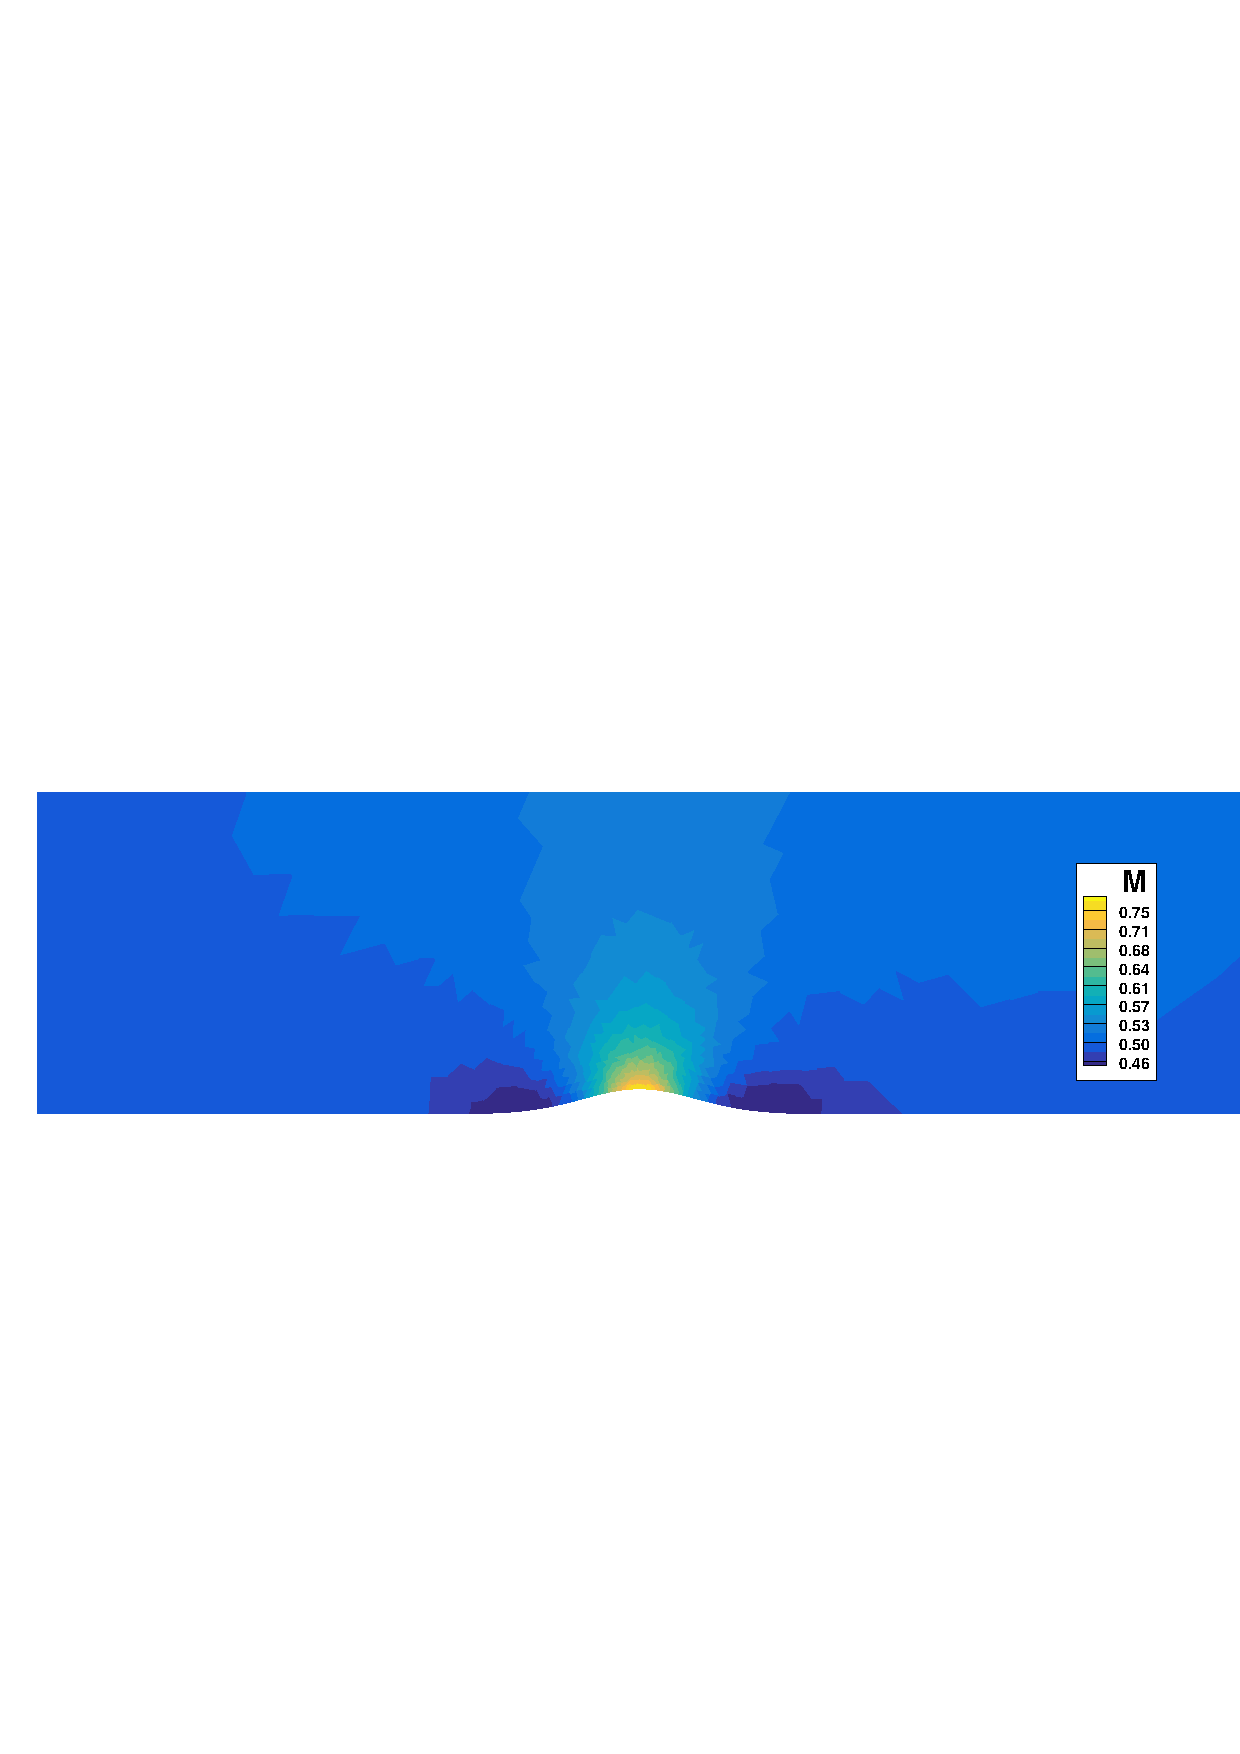
\includegraphics[width=0.85\textwidth,keepaspectratio]{machp0.png}}\\

		\hline
		\multicolumn{2}{@{}c@{}}{1st-Order Basis ($p=1$)}\\
		\hline

		\multicolumn{2}{@{}c@{}}{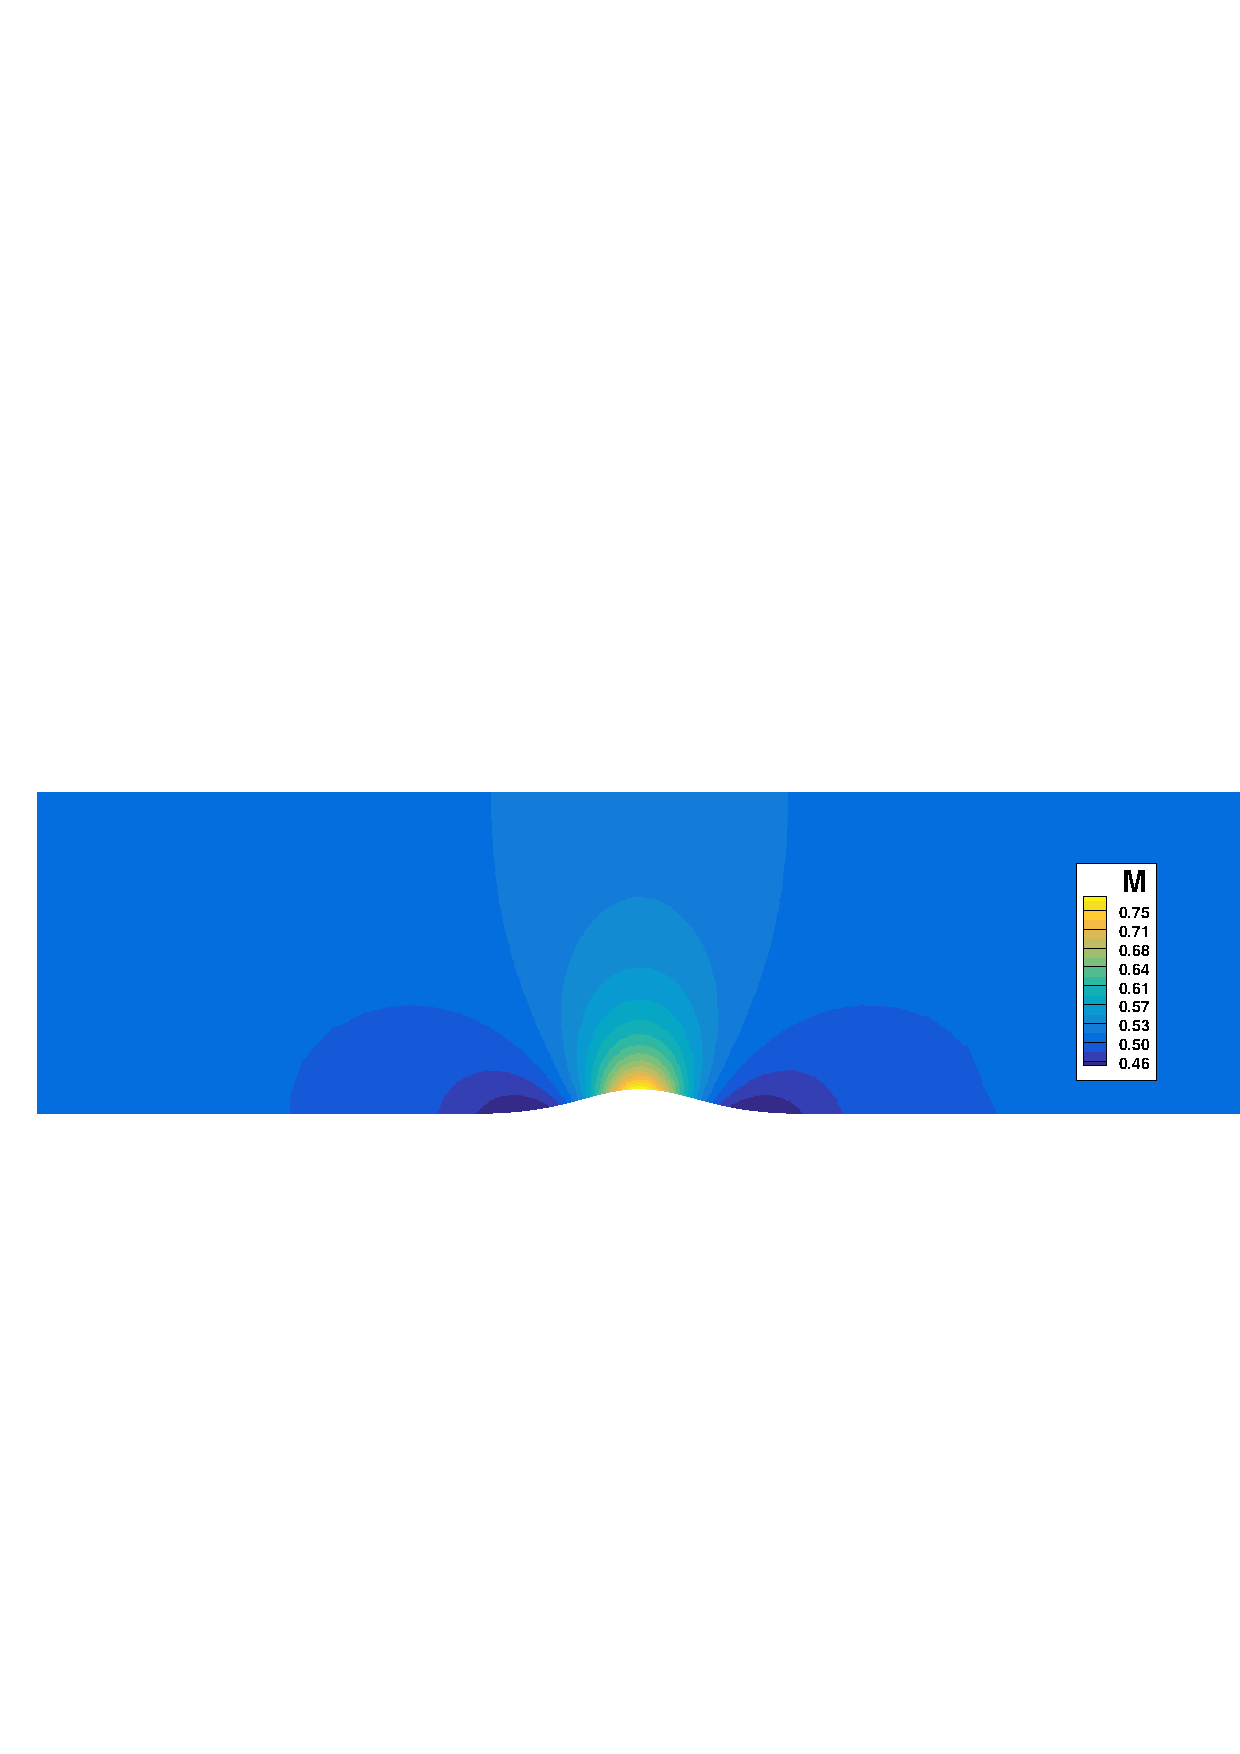
\includegraphics[width=0.85\textwidth,keepaspectratio]{machp1.png}}\\
		\hline
		\multicolumn{2}{@{}c@{}}{2nd-Order Basis ($p=2$)}\\
		\hline
		% \vspace{0.01pt}\\

		\multicolumn{2}{@{}c@{}}{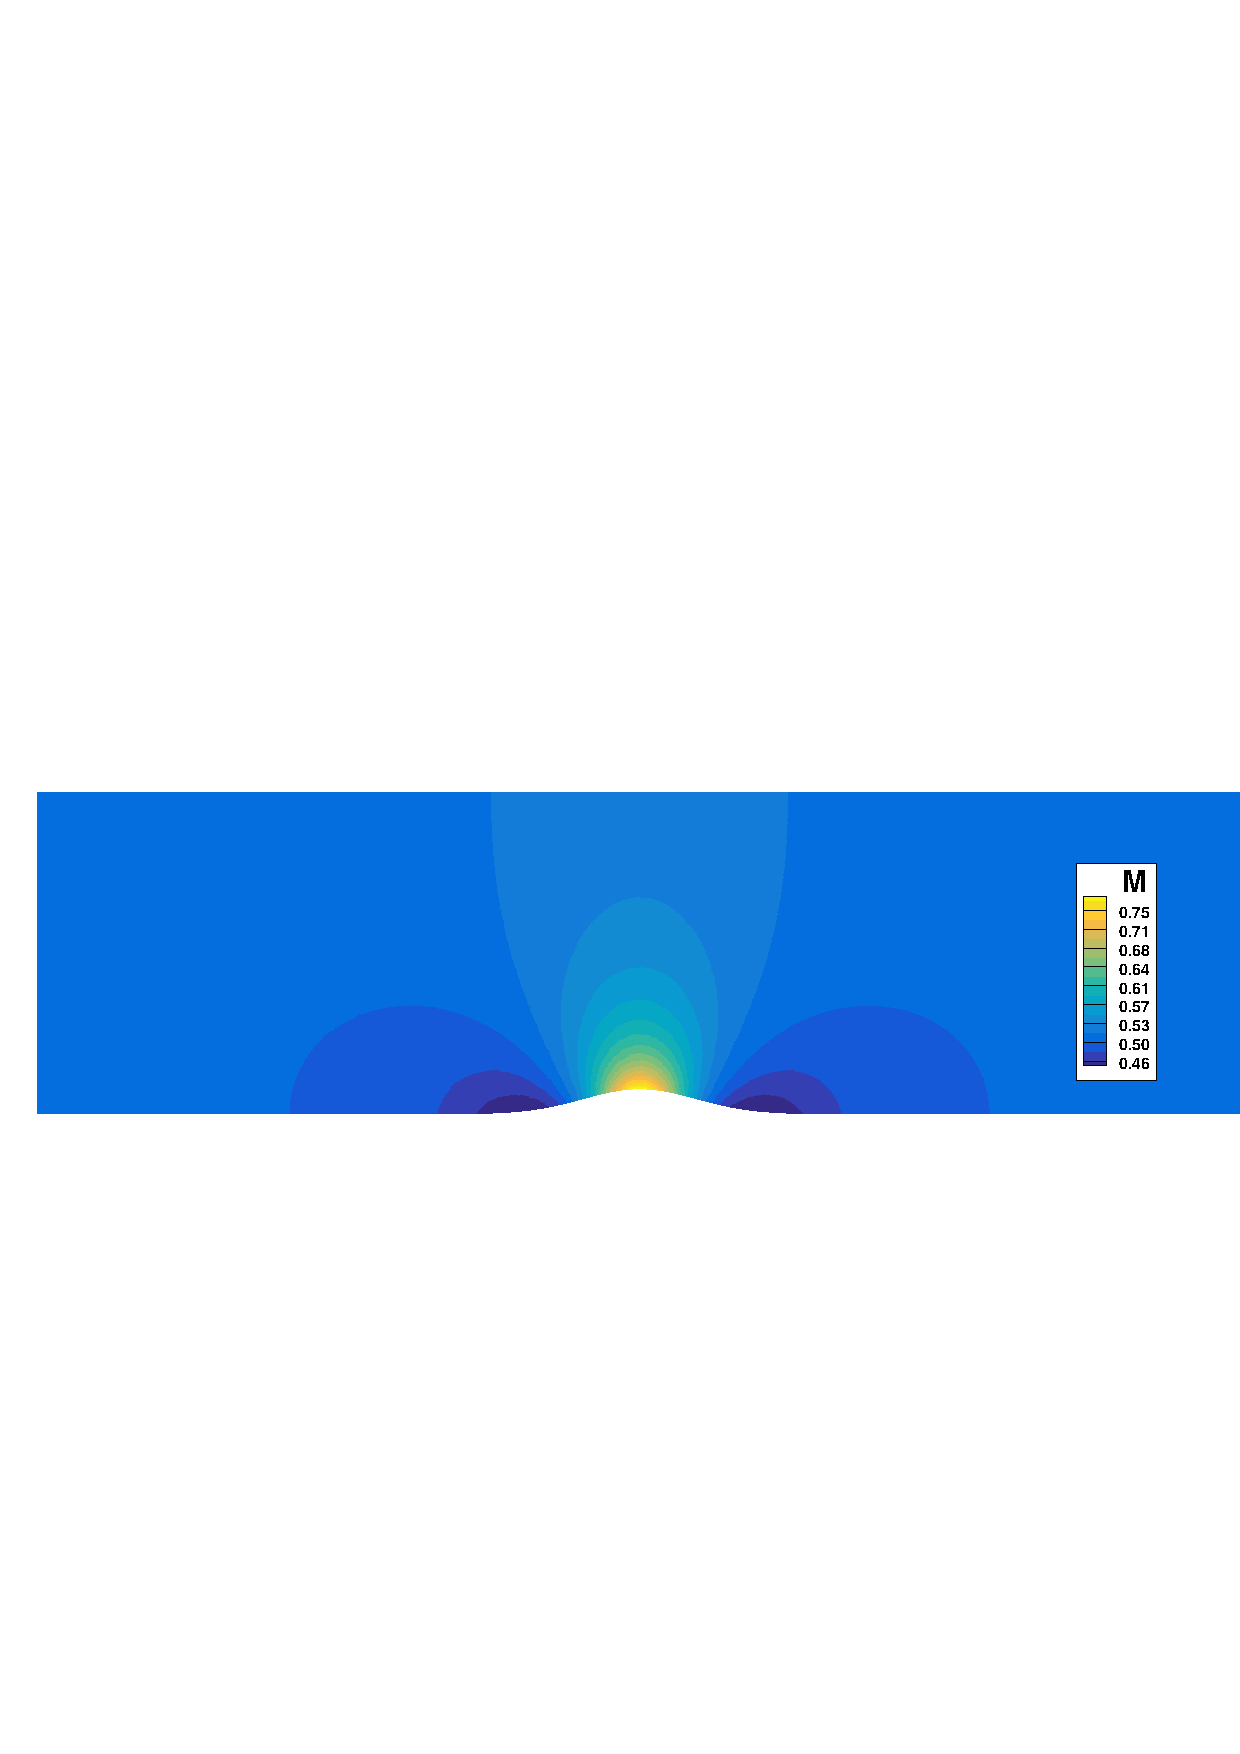
\includegraphics[width=0.85\textwidth,keepaspectratio]{machp2.png}}\\
		% \vspace{0.25mm}\\
	\end{tabular}
	\caption{\texttt{bump2.gri} Mach contours for each method}
	\label{tab:mach}
	\vspace*{-3mm}
	\end{center}
\end{table}

\subsection{Comparison with Finite Volume Method}
Figures \ref{fig:comp_cl}, \ref{fig:comp_cd}, \ref{fig:comp_Es} show the converge of the output parameters for both the DG and finite volume methods (FVM).

The 0th-order basis DG and the 1st order FVM are nearly identical of all outputs.
However, the  1st order FVM solution is slightly faster to compute, as shown in Figure \ref{fig:comp_walltime}.
Although, because the 1st order FVM outputs converge so slowly it is unlike to ever be a benefit in practice.
Otherwise, the DG method does as good or better than the FVM in terms of all other outputs and runtime!
Although it was more work to implement, the DG method offers greater levels of accuracy for a given run time and  more flexibility in terms of the desired order of accuracy.

\begin{figure}[H]
	\centering
	\includegraphics[width=0.60\textwidth,keepaspectratio]{comp_cd.png}
	\caption{The DG and FVM methods predict $C_d$ similarly for a given number of dof}
\label{fig:comp_cl}
\end{figure}
\begin{figure}[H]
\centering
\includegraphics[width=0.60\textwidth,keepaspectratio]{comp_cl.png}
\caption{The high-order DG methods predict $C_l$ more accurately}
\label{fig:comp_cd}
\end{figure}
\begin{figure}[H]
\centering
\includegraphics[width=0.60\textwidth,keepaspectratio]{comp_Es.png}
\caption{The higher-order DG methods tend toward zero total entropy at a faster rate than the FVM}
\label{fig:comp_Es}
\end{figure}


\begin{figure}[H]
	\centering
	\includegraphics[width=0.60\textwidth,keepaspectratio]{comp_walltime.png}
	\caption{The highest-order DG methods is the quickest for a desired level of accuracy}
	\label{fig:comp_walltime}
\end{figure}




% \bibliography{references}

\end{document}

